\documentclass[12pt,addpoints,answers]{exam}
\unframedsolutions
\renewcommand{\solutiontitle}{\noindent\textbf{Solution:}\par\noindent}
\SolutionEmphasis{\color{blue}}
%\noprintanswers
\usepackage[utf8]{inputenc}

\usepackage{booktabs}
\usepackage{tabularx}
\usepackage{multirow}
\usepackage{colortbl}
\usepackage{subcaption}
\usepackage{hyperref}
\usepackage{mathtools}
\usepackage{logicproof}
\usepackage[inline]{enumitem}
\usepackage{graphbox}
\usepackage{xfrac}
\usepackage{xspace}
\usepackage{bm}
\usepackage{tikz}
\usepackage{siunitx}

\usetikzlibrary{decorations}
\usetikzlibrary{decorations.pathreplacing}
\usetikzlibrary{positioning}
\usetikzlibrary{backgrounds}
\usetikzlibrary{matrix}
\usetikzlibrary{fit}
\usetikzlibrary{calc}
\usetikzlibrary{arrows}
\usetikzlibrary{shapes.geometric}
\usetikzlibrary{shapes.multipart}

\tikzset{
    position/.style args={#1:#2 from #3}{
        at=(#3.#1), anchor=#1+180, shift=(#1:#2)
    }
}

% Used for code embed in problem 12
\usepackage{listings}
\usepackage{color}
\usepackage{amsmath}

\usepackage{float}

\setlength{\parindent}{0em}
\setlength{\parskip}{1em}

\DeclarePairedDelimiter{\abs}{\lvert}{\rvert}
\DeclarePairedDelimiter{\lvec}{\left\langle}{\right\rangle}
\DeclareMathOperator{\sign}{sign}
\DeclareMathOperator*{\argmax}{arg\,max}
\DeclareMathOperator*{\argmin}{arg\,min}

\newcommand{\astar}{A{\small{*}}\xspace}

\pagestyle{headandfoot}
\firstpageheader{\textbf{CS4461/EE4272}}{\textbf{Final Exam}}{\textbf{April 26th--April 28th, 2020}}
\firstpageheadrule
\firstpagefooter{}{}{Page \thepage\ of \numpages}
\firstpagefootrule
\runningfooter{}{}{Page \thepage\ of \numpages}
\runningfootrule

\begin{document}
\vspace*{0.25in}
\begin{center}\Large{Exam Policies}\end{center}
\begin{itemize}
\item You will have a total of 72 hours to complete the exam: the exam releases at 12:00am on April 26th and the exam is due via submission to Canvas at 11:59pm on April 28th.
\item You \textbf{may} use the textbook, the slides, your notes... any course material is fair game.
\item You \textbf{may not} cooperate with anyone else. This is a chance to prove \textbf{your} knowledge.
\item Use of calculators is fine for checking your answers. The same is true for programs that you may write yourself, or programs that you have written for this class. \textbf{You are still expected to show your work!}
\item This is designed as a typical exam, so it is designed for a 2 hour block of time to be taken in one sitting. I am giving you four days so that each of you can find your own time to work on the exam and to prepare your solutions for submission.
\item You are free to take as much time as you wish for the exam, but you should allocate at least 2 hours for completing your answers, and more if you need to type them up.
\item \textbf{Read questions in their entirety.}\\Questions may require multiple responses, including an explanation or a justification.
\end{itemize}
\vfill
\begin{center}\Large{Nondisclosure Agreement}\end{center}
\begin{itemize}
\item I attest that I am the person taking the exam.
\item I understand that I am on my honor to do my own work without any assistance from others or outside sources not allowed and agree that I will not disclose the contents of this exam.
\item If I am discovered to have compromised the exam in any way, I understand that I will receive a zero for the exam and will be referred to the Office of Student Affairs for violation of university policies regarding academic integrity.
\end{itemize}
\vspace*{0.25in}
\hrule
\vspace*{0.25in}
\textbf{By submitting this exam, I affirm that I have read, understand, and agree to the policies of this exam and the terms this agreement.}
\vspace*{0.25in}
\newpage

\begin{questions}

%%%
%%%
\bonusquestion \textbf{(bonus)} Wireless transmissions present many challenging problems, due to the widely shared medium. One example is the problem of collision detection and/or avoidance. Name and describe the two types of node arrangements which illustrate why collision detection can not be done effectively in wireless networks.
\begin{solution}[10em]
\end{solution}
\vfill

%%%
%%%
\question[4] One of the link layer's responsibilities is error detection and/or correction. Why might the link layer want to provide detection when there is already error detection at both the network layer (IP) and the transport layer (TCP/UDP)?
\begin{solution}[10em]
	The link layer would ideally want to have error detection and correction capabilities so that it can catch errors early on in the sending process.  In order for the TCP/UDP to recognize an error has happened it needs to arrive at the endpoint, which could be many node hops away.  By having basic detection and/or correction in the link layer we can sometimes find corrupted packets which we can ask for from the previous node.  Making it so it only takes one hop to replace a corrupted packet, instead of having to travel the entire endpoint to endpoint distance.
\end{solution}
\vfill

%%%
%%%
\question[6] A given Ethernet device has experienced 6 collisions. What are the maximum and minimum possible intervals that device might wait before attempted to transmit again? Show your work!
\begin{solution}[10em]
	
\end{solution}
\vfill

%%%
%%%
\newpage
\question Consider the following extended LAN consisting of a set of bridges: B1--B7. The bridges have identified the spanning tree indicated by the given port designations.
\begin{center}
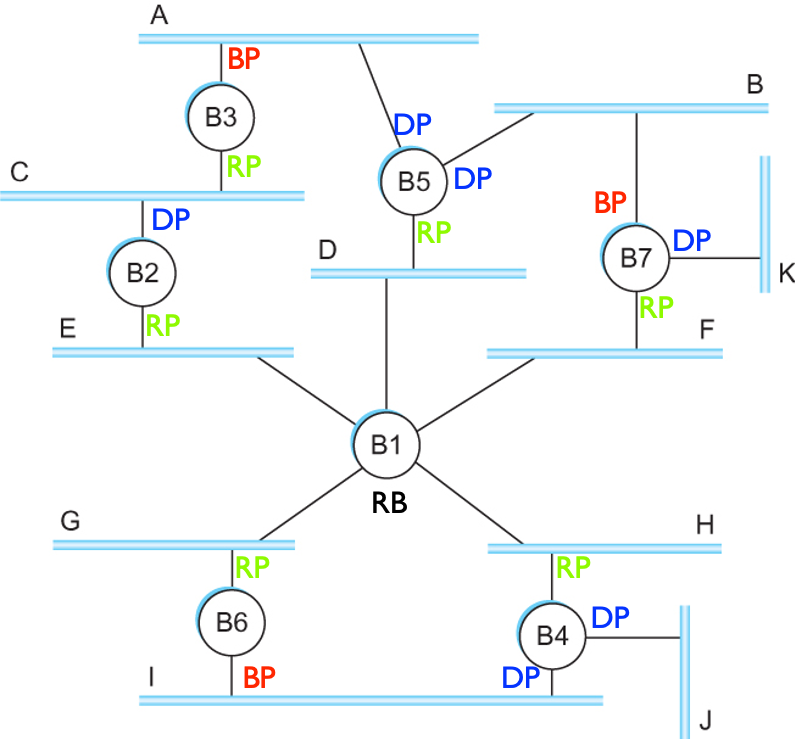
\includegraphics[width=0.3\textwidth]{fig/complex-ports.png}
\end{center}
Assume that the bridges initially have empty forwarding tables, and thus do not know where any hosts are. Further, assume that bridges will fill their forwarding table with the source address from any incoming packet, and will broadcast any packet to bridges connected via the spanning tree for which it is missing a forwarding entry. Answer the following questions about the hosts and bridges cumulatively, e.g., part (b) occurs after part (a).
\begin{parts}
\part[4] Suppose that host A1 in Ethernet A sends a TCP SYN packet destined for host J1 in Ethernet J. Which bridges learn where A1 is? Does the network interface for host K1 in Ethernet K see this packet?
\begin{solution}[10em]
	\begin{itemize}
		\item First STP Broadcast
		\begin{itemize}
			\item Bridge 5 receives broadcast from A
			\item Bridge 3 does not receive broadcast from A (Blocked Port)
		\end{itemize}
		\item Second STP Broadcast
		\begin{itemize}
			\item Bridge 7 does not receive broadcast from Bridge 5 (Blocked port)
			\item Bridge 1 receives broadcast from Bridge 5
		\end{itemize}
		\item Third STP Broadcast (Bridge 1 sends out)
		\begin{itemize}
			\item Bridge 4 receives broadcast from Bridge 1
			\item Bridge 6 receives broadcast from Bridge 1
			\item Bridge 7 receives broadcast from Bridge 1
			\item Bridge 2 receives broadcast from Bridge 1
		\end{itemize}
		\item  Fourth STP Broadcast
		\begin{itemize}
			\item Bridge 4 responds to Bridge 1 that it has J as a host
			\item Other packets still being broadcasted, but are irrelevant
		\end{itemize}
		\item Root Bridge (Bridge 1) calculates best path:
		\begin{itemize}
			\item Host A
			\item Bridge 5
			\item Bridge 1
			\item Bridge 4
			\item Host J
		\end{itemize}
	\end{itemize}

The host K1 will never see this packet, as Bridge 7 is aware that no other bridges are available on that port and it also does not have host J.  It will only send a packet up to Bridge 1 as that's the only viable path it has (is a bridge and is not blocked.)
\end{solution}

\part[4] Suppose that host J1 now sends a TCP SYN+ACK packet destined for host A1. Which bridges learn where J1 is? Does the network interface for host K1 see this packet?
\begin{solution}[10em]
\begin{itemize}
	\item First STP Broadcast
	\begin{itemize}
		\item Bridge 4 receives broadcast from J
	\end{itemize}
	\item Second STP Broadcast
	\begin{itemize}
	\item Bridge 1  receives broadcast from Bridge 4
	\end{itemize}
	\item Third STP Broadcast
	\begin{itemize}
		\item Bridge 2  receives broadcast from Bridge 1
		\item Bridge 5  receives broadcast from Bridge 1
		\item Bridge 7  receives broadcast from Bridge 1 (has nowhere to send it, and stops)
	\end{itemize}	
	\item Fourth STP Broadcast
	\begin{itemize}
		\item Bridge 3 receives broadcast from Bridge 2 (has nowhere to send it, and stops)
		\item Bridge 5 declares it has Host A available
	\end{itemize}	
	\item Fifth STP Broadcast
	\begin{itemize}
		\item Bridge 1 receives broadcast confirmation from Bridge 5 and begins calculations	
	\end{itemize}
		\item Root Bridge (Bridge 1) calculates best path:
	\begin{itemize}
		\item Host J
		\item Bridge 4
		\item Bridge 1
		\item Bridge 5
		\item Host A
	\end{itemize}
\end{itemize}
The host K1 will never see this packet, as Bridge 7 is aware that no other bridges are available on that port and it also does not have host J.  It will only send a packet up to Bridge 1 as that's the only viable path it has (is a bridge and is not blocked.)
\end{solution}


\part[4] Suppose that host E1 in Ethernet E sends a TCP SYN packet destined for host J1 in Ethernet J. Which bridges learn where E1 is? Does the network interface for host K1 in Ethernet K see this packet?
\begin{solution}[10em]
	\begin{itemize}
		\item First STP Broadcast
		\begin{itemize}
			\item Bridge 2 receives broadcast from E
			\item Bridge 1 receives broadcast from E
		\end{itemize}
		\item Second STP Broadcast
		\begin{itemize}
			\item Bridge 3 receives broadcast from Bridge 2 (has nowhere to send it, and stops)
			\item Bridge 6 receives broadcast from Bridge 1 (has nowhere to send it, and stops
			\item Bridge 7 receives broadcast from Bridge 1 (has nowhere to send it, and stops
			\item Bridge 5 receives broadcast from Bridge 1 (has nowhere to send it, and stops
			\item Bridge 4 receives broadcast from Bridge 1 and acknowledges it has host J
		\end{itemize}
		\item Third STP Broadcast
		\begin{itemize}
			\item Bridge 1 receives broadcast acknowledgment from Bridge 4 and begins to calculate
		\end{itemize}
		\item Root Bridge (Bridge 1) calculates best path:
		\begin{itemize}
			\item Host E
			\item Bridge 1
			\item Bridge 4
			\item Host J
		\end{itemize}
	\end{itemize}
\end{solution}
\vfill
\part[4] Suppose that host A1 now sends a TCP ACK packet destined for host J1. Assuming that all devices on an Ethernet are connected to a common medium (that is, they are all patched in on a single cable), does host D1 in Ethernet D see this packet?
\begin{solution}[10em]
	No, host D should not see this as STP should only be broadcasting to other bridges.  It should not need to send a broadcast to any individual host unless that host is the destination.
\end{solution}
\vfill
\end{parts}

%%%
%%%
\question[6] Complete the two-dimensional parity for the following message:
\begin{center}
\begin{tabular}{c}
\textbf{Binary} \\
\midrule
\texttt{1101110} \\
\texttt{0101011} \\
\texttt{0110001} \\
\texttt{0000000}
\end{tabular}
\end{center}
\begin{solution}[10em]
	\begin{table}[H]
		\centering
		\caption{Problem 5}
		\label{Problem 5}
		\begin{tabular}{lllllll|l}
			\cline{8-8}
			1 & 1 & 0 & 1 & 1 & 1 & 0 & \multicolumn{1}{l|}{1} \\ \cline{8-8} 
			0 & 1 & 0 & 1 & 0 & 1 & 1 & \multicolumn{1}{l|}{0} \\ \cline{8-8} 
			0 & 1 & 1 & 0 & 0 & 0 & 1 & \multicolumn{1}{l|}{1} \\ \cline{8-8} 
			0 & 0 & 0 & 0 & 0 & 0 & 0 & \multicolumn{1}{l|}{0} \\ \hline
			\multicolumn{1}{|l|}{1} & \multicolumn{1}{l|}{1} & \multicolumn{1}{l|}{1} & \multicolumn{1}{l|}{0} & \multicolumn{1}{l|}{1} & \multicolumn{1}{l|}{0} & 0 &  \\ \cline{1-7}
		\end{tabular}
	\end{table}
\end{solution}
\vfill\vfill

%%%
%%%
\newpage
\question[6] You have received the following message from a friend:
\begin{center}
\begin{tabular}{c|c}
\texttt{\textbf{0}} & \texttt{1101100} \\
\texttt{\textbf{1}} & \texttt{1100101} \\ % off
\texttt{\textbf{0}} & \texttt{1100011} \\
\texttt{\textbf{1}} & \texttt{1101011} \\
\texttt{\textbf{0}} & \texttt{0100001} \\\midrule
\texttt{\textbf{0}} & \textbf{\texttt{0110000}}
\end{tabular}
\end{center}
which you have already split up between two-dimensional parity bits and message bits. You know that the transmission line has been acting up, and you suspect there is a single bit error. Luckily, two-dimensional parity can detect and correct single bit errors! Using the mismatch between message and parity bits, identify which bit is in error.
\begin{solution}[10em]
	Row 2 column 3 is a zero where it should be a one.
	
	We can state this as Row 2 has 4 bits flipped on yet it shows that it should be an odd number.  Pair this with Column 3 has no bits flipped on, yet shows an odd number of bits should exist.  It's also much more likely that this one bit matrix[2][3] is incorrect rather than the two parity bits both being incorrect in such a fashion.
\end{solution}
\vfill

%%%
%%%
\question[4] For the values $A = 11001100_2$, $B = 10110011_2$, and $C = 10000000_2$, calculate the 8-bit 1's complement checksum for the message consisting of $A$, $B$, and $C$.\\\emph{Hint: this is the same procedure as our UDP/IP checksums, just on a shorter message.}
\begin{solution}[10em]
\end{solution}
\vfill

%%%
%%%
\newpage
\question[8] You wish to send a message $10001111_2$ across a link, where the link layer protocol uses CRC checksums generated by polynomial $x^4+x+1$. Calculate the transmitted CRC value for the message.
\begin{solution}[10em]
\end{solution}
\vfill

%%%
%%%
\question[5] Consider a path between two hosts that has 5 switches, and thus 6 links. Ignoring propagation delay, if the bitrate is \SI{1}{Mbps} and every packet on this link is \SI{1500}{bytes}, how long, in milliseconds, would it take to send 23 packets?\\\emph{Hint: remember that each packet is sent with store-and-forward, so it is incorrect to treat the transmission as one large unit.}
\begin{solution}[10em]
\end{solution}
\vfill

%%%
%%%
\newpage
\question[5] At its most distant, the planet Venus is 261 million kilometers from Earth. Consider that a new probe is collecting data about the atmosphere of Venus and wishes to send a signal with its findings back to Earth. Assuming the signal is sent at the speed of light ($\SI{3e8}{\meter/\second}$), what is the RTT for this connection based solely on the propagation delay?
\begin{solution}[10em]
\end{solution}
\vfill

%%%
%%%
\question[8] Describe completely the three messages of the famous TCP handshake used to establish a new TCP connection.
\begin{solution}[10em]
	 "Hi, I'd like to hear a TCP joke."
	
	"Hello, would you like to hear a TCP joke?"
	
	"Yes, I'd like to hear a TCP joke."
	
	"OK, I'll tell you a TCP joke."
	
	"Ok, I will hear a TCP joke."
	
	"Are you ready to hear a TCP joke?"
	
	"Yes, I am ready to hear a TCP joke."
	
	"Ok, I am about to send the TCP joke. It will last 10 seconds, it has two characters, it does not have a setting, it ends with a punchline."
	
	"Ok, I am ready to get your TCP joke that will last 10 seconds, has two characters, does not have an explicit setting, and ends with a punchline."
	
	"I'm sorry, your connection has timed out. Hello, would you like to hear a TCP joke?"
\end{solution}
\vfill

%%%
%%%
\newpage
\question Consider the following two sets of flows. For each, calculate Jain's Fairness Index.
\begin{parts}
\part[3] \SI{1000}{kbps}, \SI{780}{kbps}, \SI{100}{kbps}, \SI{810}{kbps}

\begin{center}
	Jain's Fairness Index:
\end{center}
\begin{equation}
f\left(x_{1}, x_{2}, \ldots, x_{n}\right)=\frac{\left(\sum_{i=1}^{n} x_{i}\right)^{2}}{n \sum_{i=1}^{n} x_{i}^{2}}
\end{equation}
\begin{solution}[10em]
@{from sympy import *}
@{p1Flows = [1000,780,100,810]}
@{p1FlowNumber = len(p1Flows)}
@{{{
def p1JaneDec(flows):
	val = 0
	for flow in flows:
		val += flow**2
	return val
}}}

\begin{center}
	Fairness Index:
\end{center}
$$
\frac
{
	(@{S('Sum(Symbol("f"),(i,1,4))')})^2
}
{
	n @{S('Sum(Symbol("f^2"),(i,1,4))')}
}
=
\frac
{
	@{sum(p1Flows) ** 2}
}
{
	@{p1FlowNumber * p1JaneDec(p1Flows)}
}
=
@{(sum(p1Flows) ** 2) / (p1FlowNumber * p1JaneDec(p1Flows))}
$$

\end{solution}
\vfill
\part[3] \SI{100}{kbps}, \SI{78}{kbps}, \SI{10}{kbps}, \SI{81}{kbps}
\begin{solution}[10em]
@{from sympy import *}
@{p1Flows = [100,78,10,81]}
@{p1FlowNumber = len(p1Flows)}
@{{{
def p1JaneDec(flows):
	val = 0
	for flow in flows:
		val += flow**2
	return val
}}}

\begin{center}
	Fairness Index:
\end{center}
$$
\frac
{
	(@{S('Sum(Symbol("f"),(i,1,4))')})^2
}
{
	n @{S('Sum(Symbol("f^2"),(i,1,4))')}
}
=
\frac
{
	@{sum(p1Flows) ** 2}
}
{
	@{p1FlowNumber * p1JaneDec(p1Flows)}
}
=
@{(sum(p1Flows) ** 2) / (p1FlowNumber * p1JaneDec(p1Flows))}
$$

\vspace{0.1in}

%%%%%%%%%
Calculating Jane's Fairness Index:
\definecolor{dkgreen}{rgb}{0,0.6,0}
\definecolor{gray}{rgb}{0.5,0.5,0.5}
\definecolor{mauve}{rgb}{0.58,0,0.82}
\lstset{frame=tb,
	language=Python,
	aboveskip=3mm,
	belowskip=3mm,
	showstringspaces=false,
	columns=flexible,
	basicstyle={\small\ttfamily},
	numbers=none,
	numberstyle=\tiny\color{gray},
	keywordstyle=\color{blue},
	commentstyle=\color{dkgreen},
	stringstyle=\color{mauve},
	breaklines=true,
	breakatwhitespace=true,
	tabsize=4
}
\begin{lstlisting}
p1Flows = [bandwidth_one, bandwidth_two, bandwidth_three, bandwidth_four]
p1FlowNumber = len(p1Flows)

def p1JaneDec(flows):
	val = 0
	for flow in flows:
		val += flow**2
	return val
\end{lstlisting}
\end{solution}
\vfill
\end{parts}

%%%
%%%
\question[8] Two TCP hosts are using Jacobson/Karels for timeout calculations and have been exchanging data for a long time. The current $\mathrm{EstimatedRTT}$ is \SI{18}{\milli\second} and the $\mathrm{Deviation}$ is at \SI{1}{\milli\second}. The next packet is acknowledged with an RTT of \SI{45}{\milli\second}. What are the new values of $\mathrm{EstimatedRTT}$ and $\mathrm{Timeout}$ in milliseconds? You should assume that the systems have been configured to use parameters $\delta = 0.875$, $\mu = 1$, and $\gamma = 4$.
\begin{solution}[10em]
\end{solution}
\vfill\vfill

%%%
%%%
\newpage
\question[4] The MSS for a given TCP connection is \SI{1200}{bytes}. The current Congestion Window size is \SI{1789}{bytes}. Show how the size of the Congestion Window changes when the next ACK arrives.
\begin{solution}[10em]
\end{solution}
\vfill

%%%
%%%
\question[5] Using CIDR addresses, create a forwarding table, based only on the destination address, such that:
\begin{itemize}
\item IP addresses from 192.168.10.0--192.168.15.255 are sent out port 1.
\item IP addresses from 192.168.35.0--192.168.42.255 are sent out port 2.
\item All other addresses are sent out port 3.
\end{itemize}
\begin{solution}[10em]
\begin{center}
	\begin{tabularx}{0.3\linewidth}{>{\centering\arraybackslash}Xc}
		\toprule
		\emph{CIDR Range (Destination)} & \emph{Port} \\
		\midrule
		192.168.10.0/23 & 1 \\ %  192.168.10.0 - 192.168.11.255 
		192.168.12.0/22 & 1 \\ %  192.168.12.0 - 192.168.15.255  
		192.168.35.0/24 & 2 \\ %  192.168.35.0 - 192.168.35.255
		192.168.36.0/22 & 2 \\ %  192.168.36.0 - 192.168.39.255
		192.168.40.0/23 & 2 \\ %  192.168.40.0 - 192.168.41.255
		192.168.42.0/24 & 2 \\ %  192.168.42.0 - 192.168.43.255
		0.0.0.0/0 & 3 \\ %  0.0.0.0/0 
		\bottomrule
	\end{tabularx}
\end{center}
\end{solution}
\vfill

%%%
%%%
\newpage
\question[4] A router implementing Fair Queuing is busy transmitting a packet when three flows deliver the following packets at approximately the same time. Show how those packets will be scheduled for transmission. Determine some kind of tie-breaker policy, as needed.
\begin{center}
\begin{tabular}{lccccc}
\toprule
\emph{Packet}  &  1 &  2 &  3 &  4 &  5 \\
\emph{Size}    & 45 & 55 & 55 & 15 & 75 \\
\emph{Arrival} & 10 & 15 &  0 & 10 &  0 \\
\emph{Flow}    &  1 &  1 &  2 &  2 &  3 \\
\bottomrule
\end{tabular}
\end{center}
\begin{solution}[10em]
\end{solution}
\vfill

%%%
%%%
\question[5] An IP datagram with a payload of \SI{975} bytes (not including IP headers) is launced on a network with an MTU of \SI{772}{bytes}. Determine how many fragments are created, how big is the payload of each, what is the status of the "more" bit, and what is the value of the $\mathrm{Offset}$ field?
\begin{solution}[10em]
\end{solution}
\vfill

\end{questions}

\newpage
\begin{center}\hrulefill\\\textcolor{gray}{Scratch Work}\end{center}
\vfill

\newpage
\begin{center}\hrulefill\\\textcolor{gray}{Scratch Work}\end{center}
\vfill
\begin{center}\gradetable[v][questions]\end{center}

\end{document}
